% ==============================================================================
\section{Introduction}
\label{sec:intro}
% ==============================================================================

In modern High-Performance Computing (HPC) systems, Input/Output (I/O) throughput has become as
critical to overall efficiency as computational capability itself. As supercomputing architectures
advance toward and beyond the exascale threshold, computational throughput has increased exponentially.
However, persistent storage bandwidth has lagged behind, widening the compute-to-I/O performance gap.
For instance, Figure~\ref{fig:io_per_flop} shows how the ratio between I/O bandwidth and compute power
has evolved over the past two decades for the machines listed in the TOP500~\cite{top500} and
IO500~\cite{io500list} rankings. Since 2000, the I/O bandwidth available per unit of compute has
dropped by roughly $50\times$, from 312~GB/s per PFlop/s on ASCI Red down to 6.0~GB/s per PFlop/s
on Frontier, with only a modest recovery on the more recent Aurora system.

Therefore, while modern processors achieve multi-petaflop or exaflop performance, Parallel File Systems (PFS) typically deliver only hundreds of gigabytes to a few terabytes per second in aggregate
write bandwidth. This growing imbalance creates a severe bottleneck: high-performance computing
tasks spend a non-negligible fraction of their allocated runtime waiting for data transfers to
complete.

\begin{figure}[h]
  \centering
  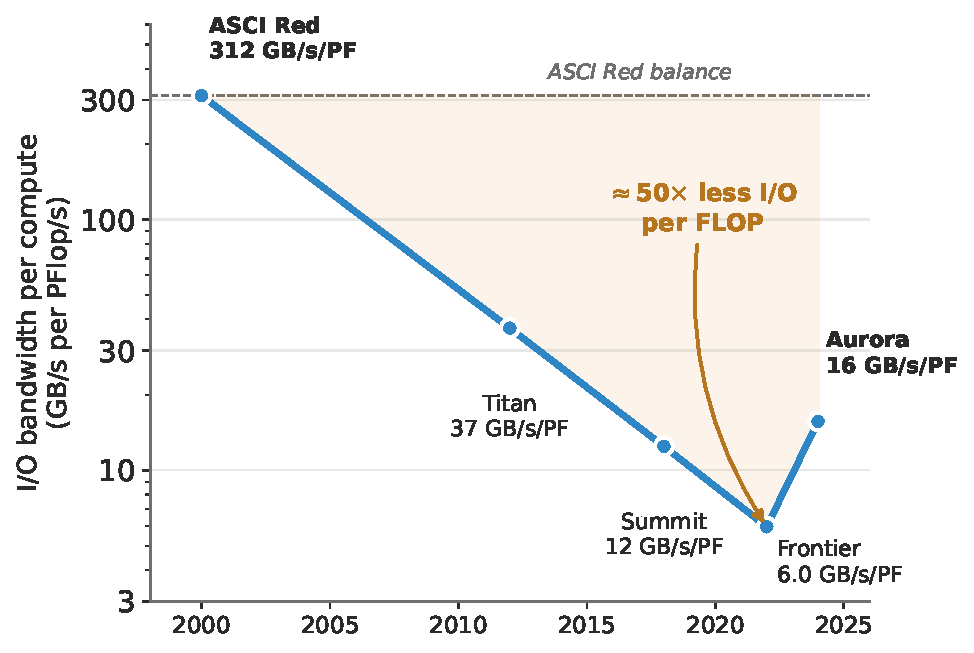
\includegraphics[width=0.55\textwidth]{figures/io_per_flop.pdf}
  \caption{Compute-to-I/O performance gap in Top500 supercomputers (2000--2025). The ratio of
  storage bandwidth per unit of compute has degraded by more than an order of magnitude.}
  \label{fig:io_per_flop}
\end{figure}

Large-scale scientific simulations generate massive volumes of data requiring efficient parallel
management. On shared PFS, thousands of concurrent processes must
coordinate access to shared storage arrays while contending for network link bandwidth and storage
controller resources. An example of an application with strong I/O pressure is \textsc{Gysela}%
~\cite{grandgirard2016gysela}, a 5D gyrokinetic code developed at CEA/IRFM
(\textit{Commissariat à l'Énergie Atomique et aux Énergies Alternatives}) for nuclear fusion
research. It models plasma turbulence in magnetic confinement devices (tokamaks) by evolving a
distribution function over three space coordinates and two velocity coordinates. At production
scale, this function reaches about 2~TB. A simulation runs for days to weeks, on hundreds to
thousands of nodes, as a chain of runs. Only low-dimensional diagnostics are saved along the way,
while the full distribution function is written at the end of each run so that the simulation can
restart~\cite{trochon2025checkpointing}.

This checkpoint is synchronous: all processes pause the numerical integration and flush their
share of the distribution function to persistent storage. A single checkpoint can generate
terabytes of data, which puts strong pressure on the storage system and interferes with the other
applications sharing it. During this phase, compute resources remain idle. In shared production
environments, write times also vary strongly: file-per-process checkpoints of \textsc{Gysela} have
been observed to take up to 30 times longer than the fastest run~\cite{trochon2025checkpointing},
due to contention with uncoordinated jobs.

Improving checkpoint performance involves two layers. The first is the configuration of the PFS,
through layout parameters such as the stripe count (number of storage targets) and the stripe
size. The second is how the application maps its data to files. Many such mappings exist; in this
report, we consider three that we name Single Shared File, Subfiling, and File Per Process, and
that differ in coordination overhead, metadata pressure, and raw throughput. We study both layers
jointly.

Running \textsc{Gysela} itself is costly, so we use \texttt{gys\_io}~\cite{gysela_miniapp_io}, a
mini-application developed outside the main \textsc{Gysela} code base. It isolates the I/O phases
of \textsc{Gysela} and reproduces their access patterns without the physics computation, which
allows fast and reproducible parameter sweeps.

This work was carried out within the \textsc{TADaaM} research team (\textit{Topology-Aware system-scale Data
management for high-performance computing}) at the Inria Centre at the University of Bordeaux, which
specializes in designing system software and data-management layers that bridge the gap between application-level
requirements and complex hardware topologies in HPC environments. The study is framed within the NumPex program,
the French national initiative building the software ecosystem for exascale supercomputing, and more specifically within
the Exa-DOST work package, which targets advanced I/O optimization strategies and dynamic data-management middlewares
for extreme-scale applications. Collaborative ties between Inria TADaaM and CEA (\textit{Commissariat à l'Énergie Atomique et aux
Énergies Alternatives}) motivate the choice of \textsc{Gysela} as the target application: joint efforts between the two institutions
aim to prepare \textsc{Gysela}'s I/O for upcoming European exascale machines, including Alice Recoque in France.

\paragraph{Contributions.} The main contributions of this work are the following:
% TODO: revisit once final results are available
\begin{itemize}
  \item We evaluate the impact of PFS striping parameters (stripe count and stripe size) on
        checkpoint write bandwidth at production scale on Adastra.
  \item We compare three write strategies, implemented through the PDI middleware, on
        representative 5D grid configurations and process counts, and characterize how each
        depends on its parameters (notably the number of subfiles).
  \item We derive tuning guidelines for \textsc{Gysela}'s checkpoint I/O.
\end{itemize}

All performance results are obtained on the Adastra supercomputer at CINES, a production system
with a Lustre file system. Complementary experiments, at a smaller scale, are run on the
Plafrim cluster, which relies on a different PFS (BeeGFS). They validate our methodology and
show whether the trends observed on Adastra hold on another platform.

\paragraph{Organization.}
The remainder of this report is organized as follows.
Section~\ref{sec:background} reviews parallel file system concepts, data striping, and the three
write strategies under evaluation, together with the software stack used throughout our
experiments.
Section~\ref{sec:setup} details the experimental setup: the target platform, benchmark workload,
and the range of parameters explored.
Section~\ref{sec:results} presents and analyzes our performance measurements.
Section~\ref{sec:conclusion} summarizes the findings and outlines directions for future work.